% Chương 2: Background & Related Work

% ==========================================
% CHƯƠNG 2: BACKGROUND & RELATED WORK
% ==========================================
\chapter{Cơ sở lý thuyết}

Chương này trình bày kiến thức nền và công trình liên quan phục vụ cho phần thiết kế thực nghiệm ở các chương sau. Nội dung chương tập trung vào cơ chế và khái niệm, không đi sâu vào kết quả đo của hệ thống cụ thể.

\section{Cơ chế xử lý gói tin trong nhân Linux}
Trong Linux networking stack, gói tin đi qua nhiều tầng xử lý trước khi tới ứng dụng đích. Với bối cảnh Kubernetes Service 
datapath, các khái niệm nền tảng cần nắm gồm:
\subsection{Netfilter framework/ iptables và chains} iptables là công cụ cấu hình mạng hoạt động trong nhân Linux, xử lý gói tin bằng cách cho chúng đi qua các chuỗi (chains) cơ bản như PREROUTING, INPUT, OUTPUT, FORWARD, và POSTROUTING. Trong Kubernetes, kube-proxy sẽ tạo ra các chuỗi tùy chỉnh như KUBE-SERVICES (để nhận diện IP của Service) và KUBE-SEP-* (để chọn endpoint cụ thể). Quá trình tra cứu các luật (rules) trong iptables diễn ra tuần tự (linear scan), tạo ra độ phức tạp O(n). Khi có hàng ngàn Service, số lượng luật tăng lên hàng chục nghìn, khiến thời gian duyệt tăng tuyến tính và gây ra thắt cổ chai.
\subsection{DNAT và SNAT (Network Address Translation)} 
\begin{itemize}
	\item \textbf{DNAT (Destination NAT):} Khi một gói tin được gửi đến địa chỉ ảo của Service (ClusterIP), chuỗi PREROUTING sẽ áp dụng DNAT để biến đổi địa chỉ IP đích từ Service IP sang địa chỉ IP thực của một Pod backend.
	\item SNAT (Source NAT / Masquerade): Khi gói tin đi ra khỏi Pod hoặc Node, chuỗi POSTROUTING sẽ thực hiện SNAT, thay đổi địa chỉ IP nguồn từ IP của Pod thành IP của Node vật lý để che giấu (hide) địa chỉ IP nội bộ của Pod.
\end{itemize}
\subsection{Conntrack (Connection Tracking)}
Đây là một hệ thống con (subsystem) của kernel chuyên theo dõi trạng thái của các kết nối mạng (stateful inspection). Ví dụ, một gói tin TCP SYN tạo ra trạng thái NEW, và gói SYN-ACK cập nhật trạng thái thành ESTABLISHED. Bất kỳ thao tác NAT nào cũng bắt buộc phải có conntrack để ghi nhớ IP/Port gốc, từ đó giúp kernel có thể dịch ngược lại chính xác địa chỉ cho các gói tin phản hồi (reply traffic). Điểm yếu của cơ chế này là dưới mức tải cao, nếu bảng conntrack đạt đến giới hạn tối đa (bị đầy), hệ thống sẽ từ chối (DROP) các kết nối mới làm thông lượng mạng sụt giảm đột ngột.


Trong benchmark networking, tail latency thường nhạy với độ phức tạp đường đi gói tin và mức tải của các thành phần xử lý trạng thái như conntrack. Vì vậy, khi phân tích p95/p99 cần đặt kết quả trong ngữ cảnh đường đi datapath thực tế.

\section{Kubernetes networking background}
Tại mức khái niệm, Service trong Kubernetes cung cấp một virtual IP (ClusterIP) để phân phối traffic tới tập backend endpoints. kube-proxy thường đảm nhiệm phần điều hướng Service bằng cách lập trình luật iptables hoặc cơ chế tương đương.

Trong khi đó, CNI chịu trách nhiệm kết nối mạng cho Pod và thiết lập các thành phần dữ liệu cần thiết cho dataplane. Cilium là một CNI dựa trên eBPF, cho phép đưa một phần logic xử lý gói tin xuống kernel theo hướng lập trình được, đồng thời cung cấp khả năng quan sát luồng mạng (flow observability).

Khái niệm kube-proxy replacement của Cilium trong nghiên cứu này được hiểu là thay thế phần xử lý Service forwarding của kube-proxy bằng datapath eBPF tương ứng.

\section{Datapath comparison at concept level}
Ở mức ý niệm, hai mode được đối chiếu theo các đường đi điển hình sau:

\textbf{Mode A (kube-proxy baseline)}
\begin{itemize}
	\item client $\rightarrow$ veth $\rightarrow$ host netns $\rightarrow$ iptables/kube-proxy path $\rightarrow$ endpoint.
\end{itemize}

\textbf{Mode B (Cilium eBPF kube-proxy replacement)}
\begin{itemize}
	\item client $\rightarrow$ veth $\rightarrow$ TC eBPF $\rightarrow$ service map $\rightarrow$ endpoint/policy map.
\end{itemize}

Trong phạm vi chương này, phần so sánh chỉ nhằm mô tả background mechanism. Nghiên cứu không đưa ra tuyên bố độ phức tạp thuật toán theo dạng chứng minh hình thức.

\begin{figure}[H]
\centering
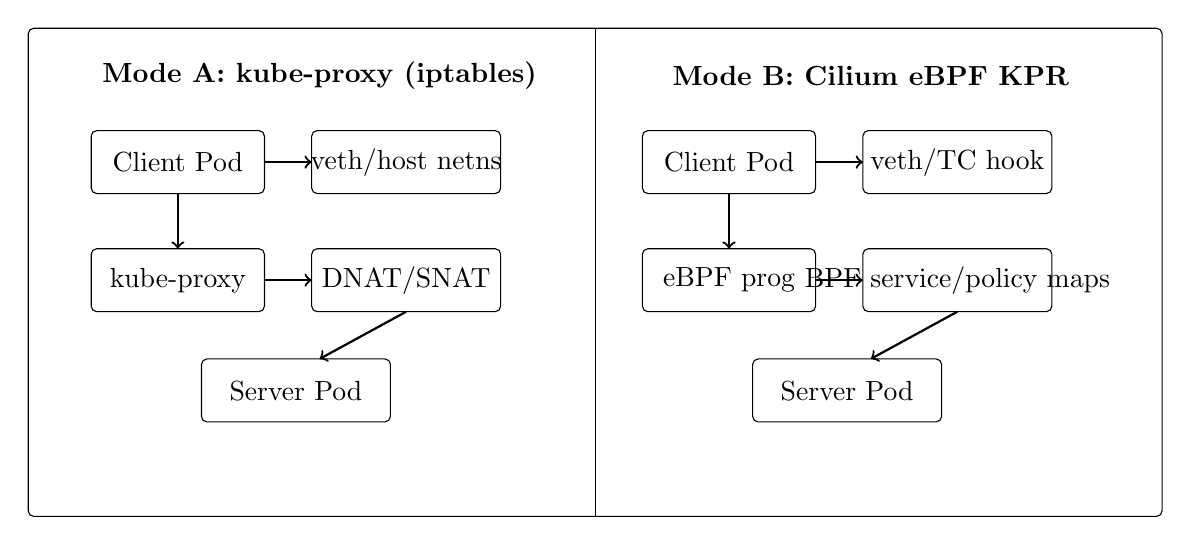
\begin{tikzpicture}[x=1cm,y=1cm]
	% Khung tổng thể
	\draw[rounded corners=2pt] (-0.2,-0.4) rectangle (14.2,5.8);
	\draw (7,-0.4) -- (7,5.8);

	% Tieu de hai cot
	\node[font=\bfseries] at (3.5,5.2) {Mode A: kube-proxy (iptables)};
	\node[font=\bfseries] at (10.5,5.2) {Mode B: Cilium eBPF KPR};

	% Mode A
	\draw[rounded corners=2pt] (0.6,3.7) rectangle (2.8,4.5);
	\node at (1.7,4.1) {Client Pod};
	\draw[rounded corners=2pt] (3.4,3.7) rectangle (5.8,4.5);
	\node at (4.6,4.1) {veth/host netns};
	\draw[rounded corners=2pt] (0.6,2.2) rectangle (2.8,3.0);
	\node at (1.7,2.6) {kube-proxy};
	\draw[rounded corners=2pt] (3.4,2.2) rectangle (5.8,3.0);
	\node at (4.6,2.6) {DNAT/SNAT};
	\draw[rounded corners=2pt] (2.0,0.8) rectangle (4.4,1.6);
	\node at (3.2,1.2) {Server Pod};

	\draw[->,thick] (2.8,4.1) -- (3.4,4.1);
	\draw[->,thick] (1.7,3.7) -- (1.7,3.0);
	\draw[->,thick] (2.8,2.6) -- (3.4,2.6);
	\draw[->,thick] (4.6,2.2) -- (3.5,1.6);

	% Mode B
	\draw[rounded corners=2pt] (7.6,3.7) rectangle (9.8,4.5);
	\node at (8.7,4.1) {Client Pod};
	\draw[rounded corners=2pt] (10.4,3.7) rectangle (12.8,4.5);
	\node at (11.6,4.1) {veth/TC hook};
	\draw[rounded corners=2pt] (7.6,2.2) rectangle (9.8,3.0);
	\node at (8.7,2.6) {eBPF prog};
	\draw[rounded corners=2pt] (10.4,2.2) rectangle (12.8,3.0);
	\node at (11.6,2.6) {BPF service/policy maps};
	\draw[rounded corners=2pt] (9.0,0.8) rectangle (11.4,1.6);
	\node at (10.2,1.2) {Server Pod};

	\draw[->,thick] (9.8,4.1) -- (10.4,4.1);
	\draw[->,thick] (8.7,3.7) -- (8.7,3.0);
	\draw[->,thick] (9.8,2.6) -- (10.4,2.6);
	\draw[->,thick] (11.6,2.2) -- (10.5,1.6);
\end{tikzpicture}
\caption{Datapath Comparison Diagram (conceptual)}
\label{fig:datapath-comparison}
\end{figure}

\section{Hubble and policy observability}
Hubble cung cấp mặt quan sát flow-level cho môi trường Cilium, bao gồm các thông tin như quan hệ nguồn-đích, metadata ngữ cảnh, và verdict của flow. Trong thesis này, Hubble được sử dụng như nguồn evidence bổ trợ thay vì thay thế số đo hiệu năng từ workload benchmark.

Các trạng thái verdict điển hình gồm \texttt{FORWARDED}/\texttt{DROPPED} và \texttt{ALLOWED}/\texttt{DENIED}. Vai trò chính của Hubble trong nghiên cứu là:
\begin{itemize}
	\item supporting evidence cho tính đúng đắn của đường đi traffic.
	\item correctness evidence khi kiểm chứng hành vi policy.
	\item bằng chứng đặc biệt quan trọng cho kịch bản S3 (policy overhead).
\end{itemize}

\section{Related work}
Tổng quan công trình liên quan được tóm tắt ở Bảng~\ref{tab:related-work-comparison}. Bảng này tập trung vào khoảng trống giữa tài liệu kỹ thuật hiện có và nhu cầu benchmark thực nghiệm có kiểm soát trên EKS.

\begin{table}[H]
\centering
\caption{Related Work Comparison}
\label{tab:related-work-comparison}
\begin{tabularx}{\textwidth}{>{\raggedright\arraybackslash}p{2.5cm}>{\raggedright\arraybackslash}p{1.9cm}X>{\raggedright\arraybackslash}p{2.8cm}>{\raggedright\arraybackslash}p{3.0cm}}
\toprule
\textbf{Nguồn} & \textbf{Môi trường} & \textbf{Nội dung chính} & \textbf{Điểm còn thiếu} & \textbf{Thesis này bổ sung} \\
\midrule
Cilium docs/benchmark notes & self-managed/cloud & Benchmark về Cilium và cơ chế datapath & Thiếu protocol đầy đủ và bộ artifact chuẩn hóa & Protocol benchmark rõ ràng, artifact provenance nhất quán \\
Kubernetes/kube-proxy docs & docs & Mô tả cơ chế Service handling và kube-proxy & Không có benchmark so sánh A/B đầy đủ trên EKS & Benchmark A/B trực tiếp trên EKS thật \\
Tài liệu Hubble & docs & Flow observability và policy verdict & Không đo policy overhead dưới workload thực nghiệm & Bổ sung S3 policy overhead kèm evidence theo flow \\
Các nguồn blog/notes cộng đồng & mixed & Kinh nghiệm thực hành và tuning thực tế & Khó tái lập, thiếu kiểm soát biến & Thiết kế thực nghiệm kiểm soát biến và phạm vi kết luận rõ ràng \\
\bottomrule
\end{tabularx}
\end{table}

\section{Scope boundary}
Để tránh over-claim, thesis xác định rõ biên phạm vi của kết luận như sau.

\textbf{Trong scope}
\begin{itemize}
	\item Service kiểu \texttt{ClusterIP}.
	\item Workload HTTP.
	\item Ưu tiên same-node theo thiết kế triển khai benchmark.
	\item Các kịch bản S1, S2, S3 như định nghĩa trong protocol.
\end{itemize}

\textbf{Ngoài scope}
\begin{itemize}
	\item Nghiên cứu đầy đủ cross-node path ở quy mô mở rộng.
	\item Service kiểu NodePort/LoadBalancer.
	\item Workload gRPC.
	\item Policy complexity scaling nhiều cấp độ.
	\item Môi trường multi-cluster.
\end{itemize}
